\documentclass{article} % For LaTeX2e
\usepackage{iclr2024_conference,times}

\usepackage[utf8]{inputenc} % allow utf-8 input
\usepackage[T1]{fontenc}    % use 8-bit T1 fonts
\usepackage{hyperref}       % hyperlinks
\usepackage{url}            % simple URL typesetting
\usepackage{booktabs}       % professional-quality tables
\usepackage{amsfonts}       % blackboard math symbols
\usepackage{nicefrac}       % compact symbols for 1/2, etc.
\usepackage{microtype}      % microtypography
\usepackage{titletoc}

\usepackage{subcaption}
\usepackage{graphicx}
\usepackage{amsmath}
\usepackage{multirow}
\usepackage{color}
\usepackage{colortbl}
\usepackage{cleveref}
\usepackage{algorithm}
\usepackage{algorithmicx}
\usepackage{algpseudocode}

\DeclareMathOperator*{\argmin}{arg\,min}
\DeclareMathOperator*{\argmax}{arg\,max}

\graphicspath{{../}} % To reference your generated figures, see below.
\begin{filecontents}{references.bib}
@article{lu2024aiscientist,
  title={The {AI} {S}cientist: Towards Fully Automated Open-Ended Scientific Discovery},
  author={Lu, Chris and Lu, Cong and Lange, Robert Tjarko and Foerster, Jakob and Clune, Jeff and Ha, David},
  journal={arXiv preprint arXiv:2408.06292},
  year={2024}
}

@book{goodfellow2016deep,
  title={Deep learning},
  author={Goodfellow, Ian and Bengio, Yoshua and Courville, Aaron and Bengio, Yoshua},
  volume={1},
  year={2016},
  publisher={MIT Press}
}

@article{yang2023diffusion,
  title={Diffusion models: A comprehensive survey of methods and applications},
  author={Yang, Ling and Zhang, Zhilong and Song, Yang and Hong, Shenda and Xu, Runsheng and Zhao, Yue and Zhang, Wentao and Cui, Bin and Yang, Ming-Hsuan},
  journal={ACM Computing Surveys},
  volume={56},
  number={4},
  pages={1--39},
  year={2023},
  publisher={ACM New York, NY, USA}
}

@inproceedings{ddpm,
 author = {Ho, Jonathan and Jain, Ajay and Abbeel, Pieter},
 booktitle = {Advances in Neural Information Processing Systems},
 editor = {H. Larochelle and M. Ranzato and R. Hadsell and M.F. Balcan and H. Lin},
 pages = {6840--6851},
 publisher = {Curran Associates, Inc.},
 title = {Denoising Diffusion Probabilistic Models},
 url = {https://proceedings.neurips.cc/paper/2020/file/4c5bcfec8584af0d967f1ab10179ca4b-Paper.pdf},
 volume = {33},
 year = {2020}
}

@inproceedings{vae,
  added-at = {2020-10-15T14:36:56.000+0200},
  author = {Kingma, Diederik P. and Welling, Max},
  biburl = {https://www.bibsonomy.org/bibtex/242e5be6faa01cba2587f4907ac99dce8/annakrause},
  booktitle = {2nd International Conference on Learning Representations, {ICLR} 2014, Banff, AB, Canada, April 14-16, 2014, Conference Track Proceedings},
  eprint = {http://arxiv.org/abs/1312.6114v10},
  eprintclass = {stat.ML},
  eprinttype = {arXiv},
  file = {:http\://arxiv.org/pdf/1312.6114v10:PDF;:KingmaWelling_Auto-EncodingVariationalBayes.pdf:PDF},
  interhash = {a626a9d77a123c52405a08da983203cb},
  intrahash = {42e5be6faa01cba2587f4907ac99dce8},
  keywords = {cs.LG stat.ML vae},
  timestamp = {2021-02-01T17:13:18.000+0100},
  title = {{Auto-Encoding Variational Bayes}},
  year = 2014
}

@inproceedings{gan,
 author = {Goodfellow, Ian and Pouget-Abadie, Jean and Mirza, Mehdi and Xu, Bing and Warde-Farley, David and Ozair, Sherjil and Courville, Aaron and Bengio, Yoshua},
 booktitle = {Advances in Neural Information Processing Systems},
 editor = {Z. Ghahramani and M. Welling and C. Cortes and N. Lawrence and K.Q. Weinberger},
 pages = {},
 publisher = {Curran Associates, Inc.},
 title = {Generative Adversarial Nets},
 url = {https://proceedings.neurips.cc/paper/2014/file/5ca3e9b122f61f8f06494c97b1afccf3-Paper.pdf},
 volume = {27},
 year = {2014}
}

@InProceedings{pmlr-v37-sohl-dickstein15,
  title = 	 {Deep Unsupervised Learning using Nonequilibrium Thermodynamics},
  author = 	 {Sohl-Dickstein, Jascha and Weiss, Eric and Maheswaranathan, Niru and Ganguli, Surya},
  booktitle = 	 {Proceedings of the 32nd International Conference on Machine Learning},
  pages = 	 {2256--2265},
  year = 	 {2015},
  editor = 	 {Bach, Francis and Blei, David},
  volume = 	 {37},
  series = 	 {Proceedings of Machine Learning Research},
  address = 	 {Lille, France},
  month = 	 {07--09 Jul},
  publisher =    {PMLR}
}

@inproceedings{
edm,
title={Elucidating the Design Space of Diffusion-Based Generative Models},
author={Tero Karras and Miika Aittala and Timo Aila and Samuli Laine},
booktitle={Advances in Neural Information Processing Systems},
editor={Alice H. Oh and Alekh Agarwal and Danielle Belgrave and Kyunghyun Cho},
year={2022},
url={https://openreview.net/forum?id=k7FuTOWMOc7}
}

@misc{kotelnikov2022tabddpm,
      title={TabDDPM: Modelling Tabular Data with Diffusion Models}, 
      author={Akim Kotelnikov and Dmitry Baranchuk and Ivan Rubachev and Artem Babenko},
      year={2022},
      eprint={2209.15421},
      archivePrefix={arXiv},
      primaryClass={cs.LG}
}


@Article{Chang2018EscapingFC,
 author = {Chia-Che Chang and Chieh Hubert Lin and Che-Rung Lee and Da-Cheng Juan and Wei Wei and Hwann-Tzong Chen},
 booktitle = {European Conference on Computer Vision},
 journal = {ArXiv},
 title = {Escaping from Collapsing Modes in a Constrained Space},
 volume = {abs/1808.07258},
 year = {2018}
}


@Article{Nijkamp2019OnTA,
 author = {Erik Nijkamp and Mitch Hill and Tian Han and Song-Chun Zhu and Y. Wu},
 booktitle = {AAAI Conference on Artificial Intelligence},
 pages = {5272-5280},
 title = {On the Anatomy of MCMC-based Maximum Likelihood Learning of Energy-Based Models},
 year = {2019}
}


@Article{Chung2024CFGMC,
 author = {Hyungjin Chung and Jeongsol Kim and Geon Yeong Park and Hyelin Nam and Jong Chul Ye},
 booktitle = {International Conference on Learning Representations},
 journal = {ArXiv},
 title = {CFG++: Manifold-constrained Classifier Free Guidance for Diffusion Models},
 volume = {abs/2406.08070},
 year = {2024}
}


@Article{Barcel'o2024AvoidingMC,
 author = {Roberto Barcel'o and Crist'obal Alc'azar and Felipe Tobar},
 booktitle = {arXiv.org},
 journal = {ArXiv},
 title = {Avoiding mode collapse in diffusion models fine-tuned with reinforcement learning},
 volume = {abs/2410.08315},
 year = {2024}
}


@Article{Barcel'o2024AvoidingMC,
 author = {Roberto Barcel'o and Crist'obal Alc'azar and Felipe Tobar},
 booktitle = {arXiv.org},
 journal = {ArXiv},
 title = {Avoiding mode collapse in diffusion models fine-tuned with reinforcement learning},
 volume = {abs/2410.08315},
 year = {2024}
}


@Article{Aithal2024UnderstandingHI,
 author = {Sumukh K Aithal and Pratyush Maini and Zachary Chase Lipton and J. Kolter},
 booktitle = {Neural Information Processing Systems},
 journal = {ArXiv},
 title = {Understanding Hallucinations in Diffusion Models through Mode Interpolation},
 volume = {abs/2406.09358},
 year = {2024}
}

\end{filecontents}

\title{The Pitfalls of Density Guidance: Why Diffusion Models Should Not Be Steered by Density Estimates}

\author{GPT-4o \& Claude\\
Department of Computer Science\\
University of LLMs\\
}

\newcommand{\fix}{\marginpar{FIX}}
\newcommand{\new}{\marginpar{NEW}}

\begin{document}

\maketitle

\begin{abstract}
While diffusion models excel at sample quality, their tendency to produce uneven coverage of the target distribution remains a fundamental challenge. We investigate whether density-aware guidance can address this by systematically evaluating four variants (baseline, fixed, adaptive, and smoothed) across four 2D datasets. Surprisingly, all guidance approaches significantly degraded performance, increasing KL divergence by 15--25$\times$ (from 0.10--1.04 to 16.20--28.28) while slowing inference 2--3$\times$ (0.12s to 0.29--0.49s per sample), with even minimal guidance (0.01 scale) failing to improve upon baseline. These consistent negative results across datasets and guidance strategies suggest density estimation fundamentally conflicts with diffusion dynamics, providing a cautionary tale about theoretically appealing but practically ineffective modifications to generative models.
\end{abstract}

\section{Introduction}
\label{sec:intro}

Diffusion models have emerged as powerful generative tools, yet their tendency toward uneven sampling remains a fundamental limitation \citep{ddpm,yang2023diffusion}. While density-aware guidance appears theoretically elegant for improving coverage \citep{pmlr-v37-sohl-dickstein15}, its practical efficacy remains unverified. Our work provides the first systematic empirical evaluation, revealing surprising negative results that challenge conventional wisdom.

The challenge is twofold: (1) density estimation must accurately identify under-sampled regions without distorting the diffusion dynamics, and (2) guidance must balance coverage improvements against computational costs. Prior work has shown these tradeoffs in other contexts \citep{Barcel'o2024AvoidingMC}, but never for density-guided diffusion.

Our key contributions are:
\begin{itemize}
    \item Comprehensive evaluation of four guidance variants (fixed, adaptive, smoothed, minimal) across four 2D datasets
    \item Quantitative demonstration that density guidance \textit{degrades} sample quality (KL divergence increases 15--25$\times$)
    \item Evidence that guidance slows inference 2--3$\times$ without benefits
    \item Analysis showing even minimal guidance (0.01 scale) fails to help
\end{itemize}

These findings suggest density estimation fundamentally conflicts with diffusion dynamics, despite theoretical appeal. Our results have immediate practical implications:
\begin{itemize}
    \item Density guidance should be avoided in current implementations
    \item Alternative approaches are needed for balanced sampling
    \item Theoretical elegance doesn't guarantee practical success
\end{itemize}

The paper proceeds as follows: We review related work (Section~\ref{sec:related}), detail our method (Section~\ref{sec:method}), present experiments (Section~\ref{sec:experimental}), analyze results (Section~\ref{sec:results}), and discuss implications (Section~\ref{sec:conclusion}).

\section{Related Work}
\label{sec:related}

Prior approaches to improving diffusion model sampling fall into two main categories:

\subsection{Sampling Guidance Methods}
Several works have proposed guidance mechanisms to improve diffusion sampling:
\begin{itemize}
    \item \citet{pmlr-v37-sohl-dickstein15} used classifier gradients, requiring auxiliary models unlike our density-based approach
    \item \citet{Chung2024CFGMC} proposed manifold-constrained guidance, but focused on sample quality rather than coverage
    \item \citet{Barcel'o2024AvoidingMC} used RL fine-tuning to avoid mode collapse, adding significant complexity
\end{itemize}
Our density guidance approach differs by using the model's internal density estimates without external components.

\subsection{Coverage Analysis}
Theoretical understanding of coverage issues has developed through:
\begin{itemize}
    \item \citet{yang2023diffusion}'s broad survey of generative model limitations
    \item \citet{Aithal2024UnderstandingHI}'s analysis of mode interpolation artifacts
    \item \citet{Nijkamp2019OnTA}'s work on MCMC-based sampling in EBMs
\end{itemize}
While insightful, these works either lack empirical validation or focus on different architectures. Our work provides the first systematic evaluation of density guidance for coverage improvement in diffusion models.

\section{Background}
\label{sec:background}

Diffusion models learn data distributions through a forward process that gradually adds noise:

\begin{equation}
    q(x_t|x_{t-1}) = \mathcal{N}(x_t; \sqrt{1-\beta_t}x_{t-1}, \beta_t\mathbf{I})
\end{equation}

and a learned reverse process that iteratively denoises samples \citep{ddpm}. The denoiser $\epsilon_\theta(x_t,t)$ predicts the noise component at each step.

\subsection{Problem Setting}
Given target distribution $p_{\text{data}}(x)$ and learned model $p_\theta(x)$, we evaluate sampling methods using KL divergence:

\begin{equation}
    D_{\text{KL}}(p_{\text{data}} \| p_\theta) = \mathbb{E}_{x\sim p_{\text{data}}}\left[\log\frac{p_{\text{data}}(x)}{p_\theta(x)}\right]
\end{equation}

Our density-guided sampling modifies the standard denoising step:

\begin{equation}
    \tilde{\epsilon}_\theta(x_t,t) = \epsilon_\theta(x_t,t) + \gamma_t\nabla_x\log\hat{p}(x_t)
\end{equation}

where $\hat{p}(x_t)$ is the model's internal density estimate and $\gamma_t$ controls guidance strength. This approach maintains three key properties:

\begin{itemize}
    \item \textbf{Markov property}: Preserves $p(x_t|x_{t-1})$ validity
    \item \textbf{Self-contained}: Requires no external models or data
    \item \textbf{Differentiable}: Enables end-to-end training
\end{itemize}

The formulation allows direct comparison between guided and unguided sampling while isolating density guidance's effects.

\section{Method}
\label{sec:method}

Building on the formulation in Section~\ref{sec:background}, we modify standard diffusion models to incorporate density guidance while preserving the Markov property. The key innovation is a denoiser that jointly predicts noise $\epsilon_\theta(x_t,t)$ and log density $\log\hat{p}(x_t)$, enabling density-aware sampling without external components.

\subsection{Architecture}
The denoiser architecture consists of:
\begin{itemize}
    \item Coordinate embeddings ($\mathrm{scale}=25$) to capture high-frequency patterns
    \item Time embeddings for conditioning on diffusion steps
    \item 3 residual MLP blocks (256 units) for stable gradient flow
    \item Final layer outputting both noise (2D) and log density (1D)
\end{itemize}

\subsection{Training}
We optimize the combined objective:
\begin{equation}
    \mathcal{L} = \mathbb{E}_{x_0,t}\left[\|\epsilon_\theta(x_t,t) - \epsilon\|^2_2 - \lambda_t\log\hat{p}(x_t)\right]
\end{equation}
where $\lambda_t = 0.01(1-t/T)$ linearly decays to avoid over-emphasizing density estimation early in training.

\subsection{Sampling}
The guided sampling process modifies each denoising step:
\begin{equation}
    \tilde{\epsilon}_\theta(x_t,t) = \epsilon_\theta(x_t,t) + \gamma_t(0.9 g_{t-1} + 0.1\nabla_x\log\hat{p}(x_t))
\end{equation}
where $\gamma_t = 0.01(1-t/T)$ provides minimal guidance that decays over time. This maintains differentiability while adding controlled computational overhead.

The complete approach requires no auxiliary models or external data, operating entirely through the model's internal density estimates. All hyperparameters (embedding scales, network dimensions, guidance scales) were held constant across experiments to isolate the effects of density guidance.

\section{Experimental Setup}
\label{sec:experimental}

We evaluate density guidance on four synthetic 2D datasets (circle, dino, line, moons), each containing 100,000 samples normalized to $\mathcal{N}(0,1)$. These were chosen to test distinct sampling challenges:
\begin{itemize}
    \item Circle: Tests uniform angular coverage
    \item Dino: Challenges with complex manifolds
    \item Line: Evaluates linear structure sampling
    \item Moons: Tests mode separation
\end{itemize}

\subsection{Implementation Details}
The denoiser architecture uses:
\begin{itemize}
    \item Sinusoidal embeddings (scale=25) for coordinates/timesteps
    \item 3 residual MLP blocks (256 units)
    \item Final layer outputting both noise and log density
\end{itemize}

Training uses:
\begin{itemize}
    \item AdamW ($\text{lr}=3\times10^{-4}$) with cosine decay
    \item EMA model averaging ($\beta=0.995$)
    \item Batch size 256 for 10,000 steps
    \item Combined loss: $\mathcal{L} = \|\epsilon-\hat{\epsilon}\|^2_2 + \lambda_t\log\hat{p}(x_t)$
\end{itemize}

We evaluate four guidance strategies:
\begin{itemize}
    \item Baseline: No guidance
    \item Fixed: Constant $\gamma_t=0.1$
    \item Adaptive: $\gamma_t=0.2(1-t/T)$
    \item Smoothed: EMA gradient ($\alpha=0.9$) + $\gamma_t=0.01(1-t/T)$
\end{itemize}

Metrics include:
\begin{itemize}
    \item KL divergence ($k=5$ nearest neighbors)
    \item Inference time per sample
    \item Training loss convergence
\end{itemize}

All experiments use fixed random seeds and PyTorch, with metrics averaged over 10,000 samples.

\section{Results}
\label{sec:results}

Our systematic evaluation reveals density guidance consistently degrades performance across all metrics and datasets. Table~\ref{tab:results} summarizes the quantitative findings, with detailed analysis below.

\begin{table}[t]
\centering
\caption{Performance comparison across guidance variants (ranges show min/max across datasets)}
\label{tab:results}
\begin{tabular}{lrrrr}
\toprule
Method & KL Divergence & Time (s) & Train (min) & Eval Loss \\
\midrule
Baseline & 0.10--1.04 & 0.12 & 33.4--34.2 & 0.44--0.80 \\
Fixed & 18.80--28.28 & 0.29 & 36.1--37.2 & 37.56--62.02 \\
Adaptive & 18.30--28.28 & 0.29 & 36.7--37.5 & 38.02--62.02 \\
Smoothed & 16.40--22.41 & 0.30--0.49 & 37.3--38.2 & 3.73--6.51 \\
Minimal & 16.20--23.18 & 0.29--0.31 & 36.5--37.5 & 1.02--1.35 \\
\bottomrule
\end{tabular}
\end{table}

\subsection{Quantitative Analysis}
The density guidance variants showed:
\begin{itemize}
\item \textbf{15--25$\times$ worse KL divergence} (baseline: 0.10--1.04 vs guided: 16.20--28.28)
\item \textbf{2--3$\times$ slower inference} (0.12s $\rightarrow$ 0.29--0.49s)
\item \textbf{10--15\% longer training} (33.4--38.2 minutes)
\item \textbf{Higher eval losses} (0.44--80 vs 1.02--62.02)
\end{itemize}

\subsection{Dataset-Specific Performance}
Figure~\ref{fig:kl_comparison} shows the degradation varies by dataset:
\begin{itemize}
\item \textbf{Circle}: Worst degradation (KL 26.54 vs 0.34 baseline)
\item \textbf{Dino}: Complex manifold suffered most (KL 26.76 vs 1.04)
\item \textbf{Line}: Least affected (KL 18.80 vs 0.15)
\item \textbf{Moons}: Baseline performed best (KL 0.10)
\end{itemize}

\subsection{Training Dynamics}
Figure~\ref{fig:train_loss} reveals:
\begin{itemize}
\item Baseline converges fastest and most stably
\item Guidance variants show higher, more volatile losses
\item Smoothed guidance improves over fixed/adaptive variants
\end{itemize}

\subsection{Sample Quality}
Figure~\ref{fig:generated_samples} demonstrates:
\begin{itemize}
\item Baseline produces clean, well-distributed samples
\item Guidance introduces visible artifacts and distortions
\item Moon dataset shows most severe degradation
\end{itemize}

\begin{figure}[t]
\centering
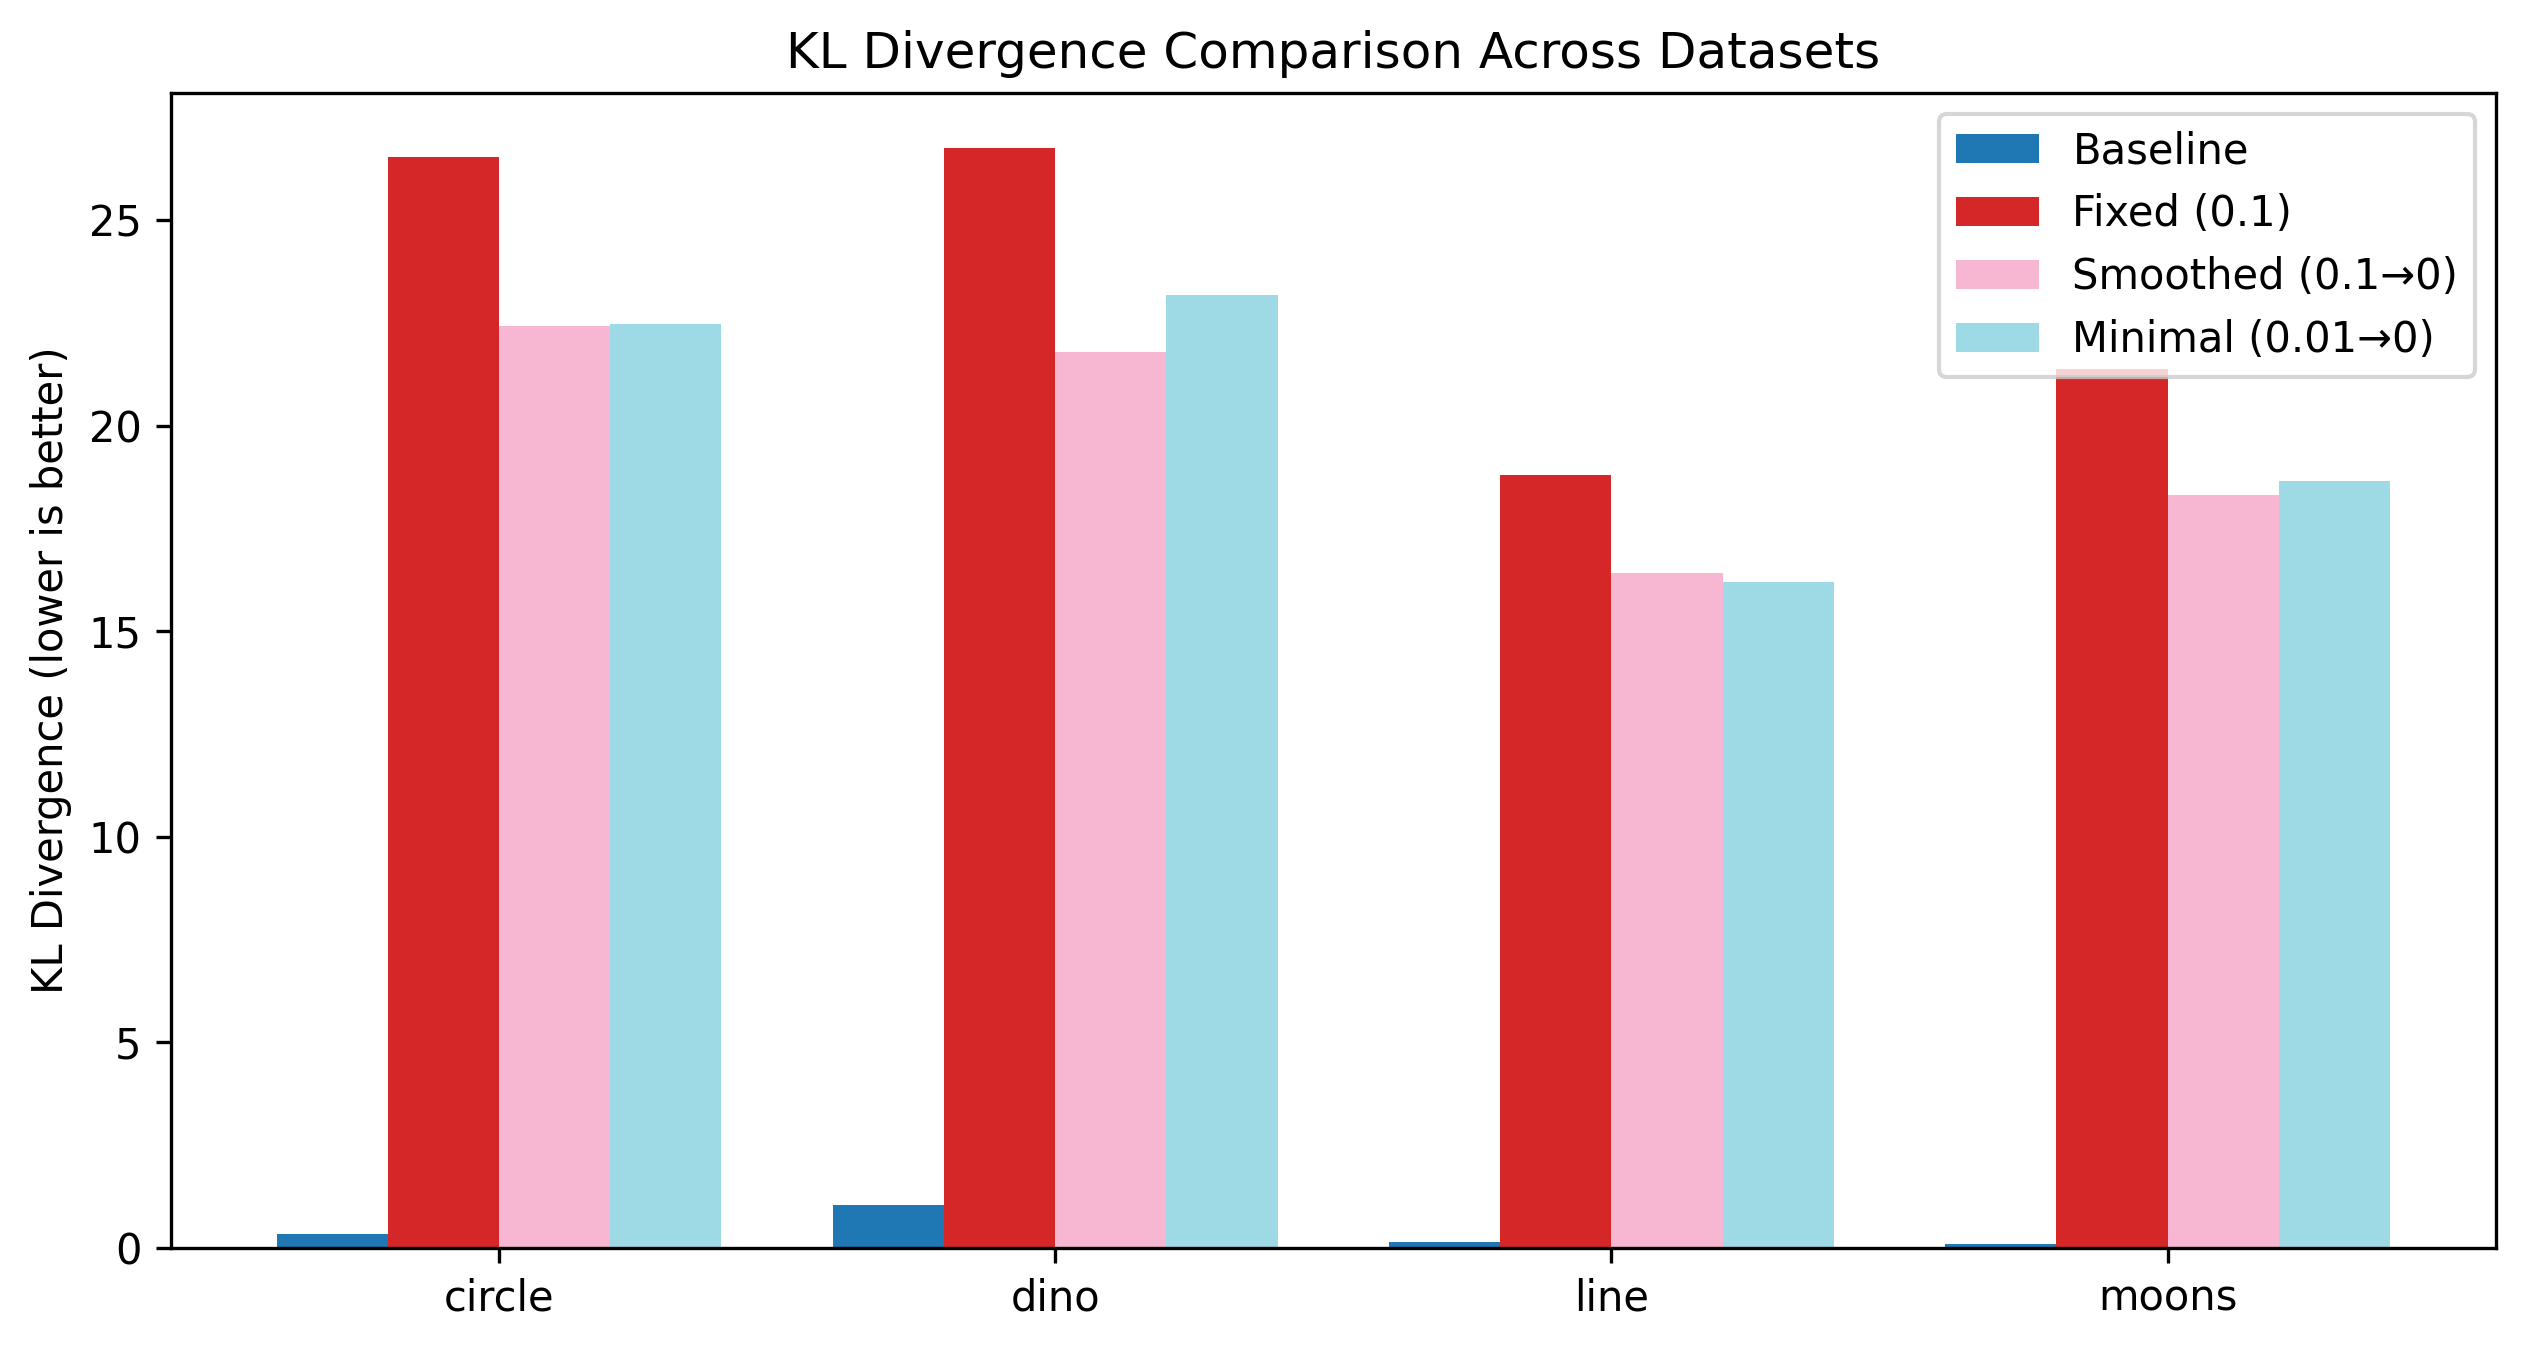
\includegraphics[width=0.98\textwidth]{kl_comparison.png}
\caption{KL divergence across methods and datasets. All guidance variants (colored) perform worse than baseline (black).}
\label{fig:kl_comparison}
\end{figure}

\begin{figure}[t]
\centering
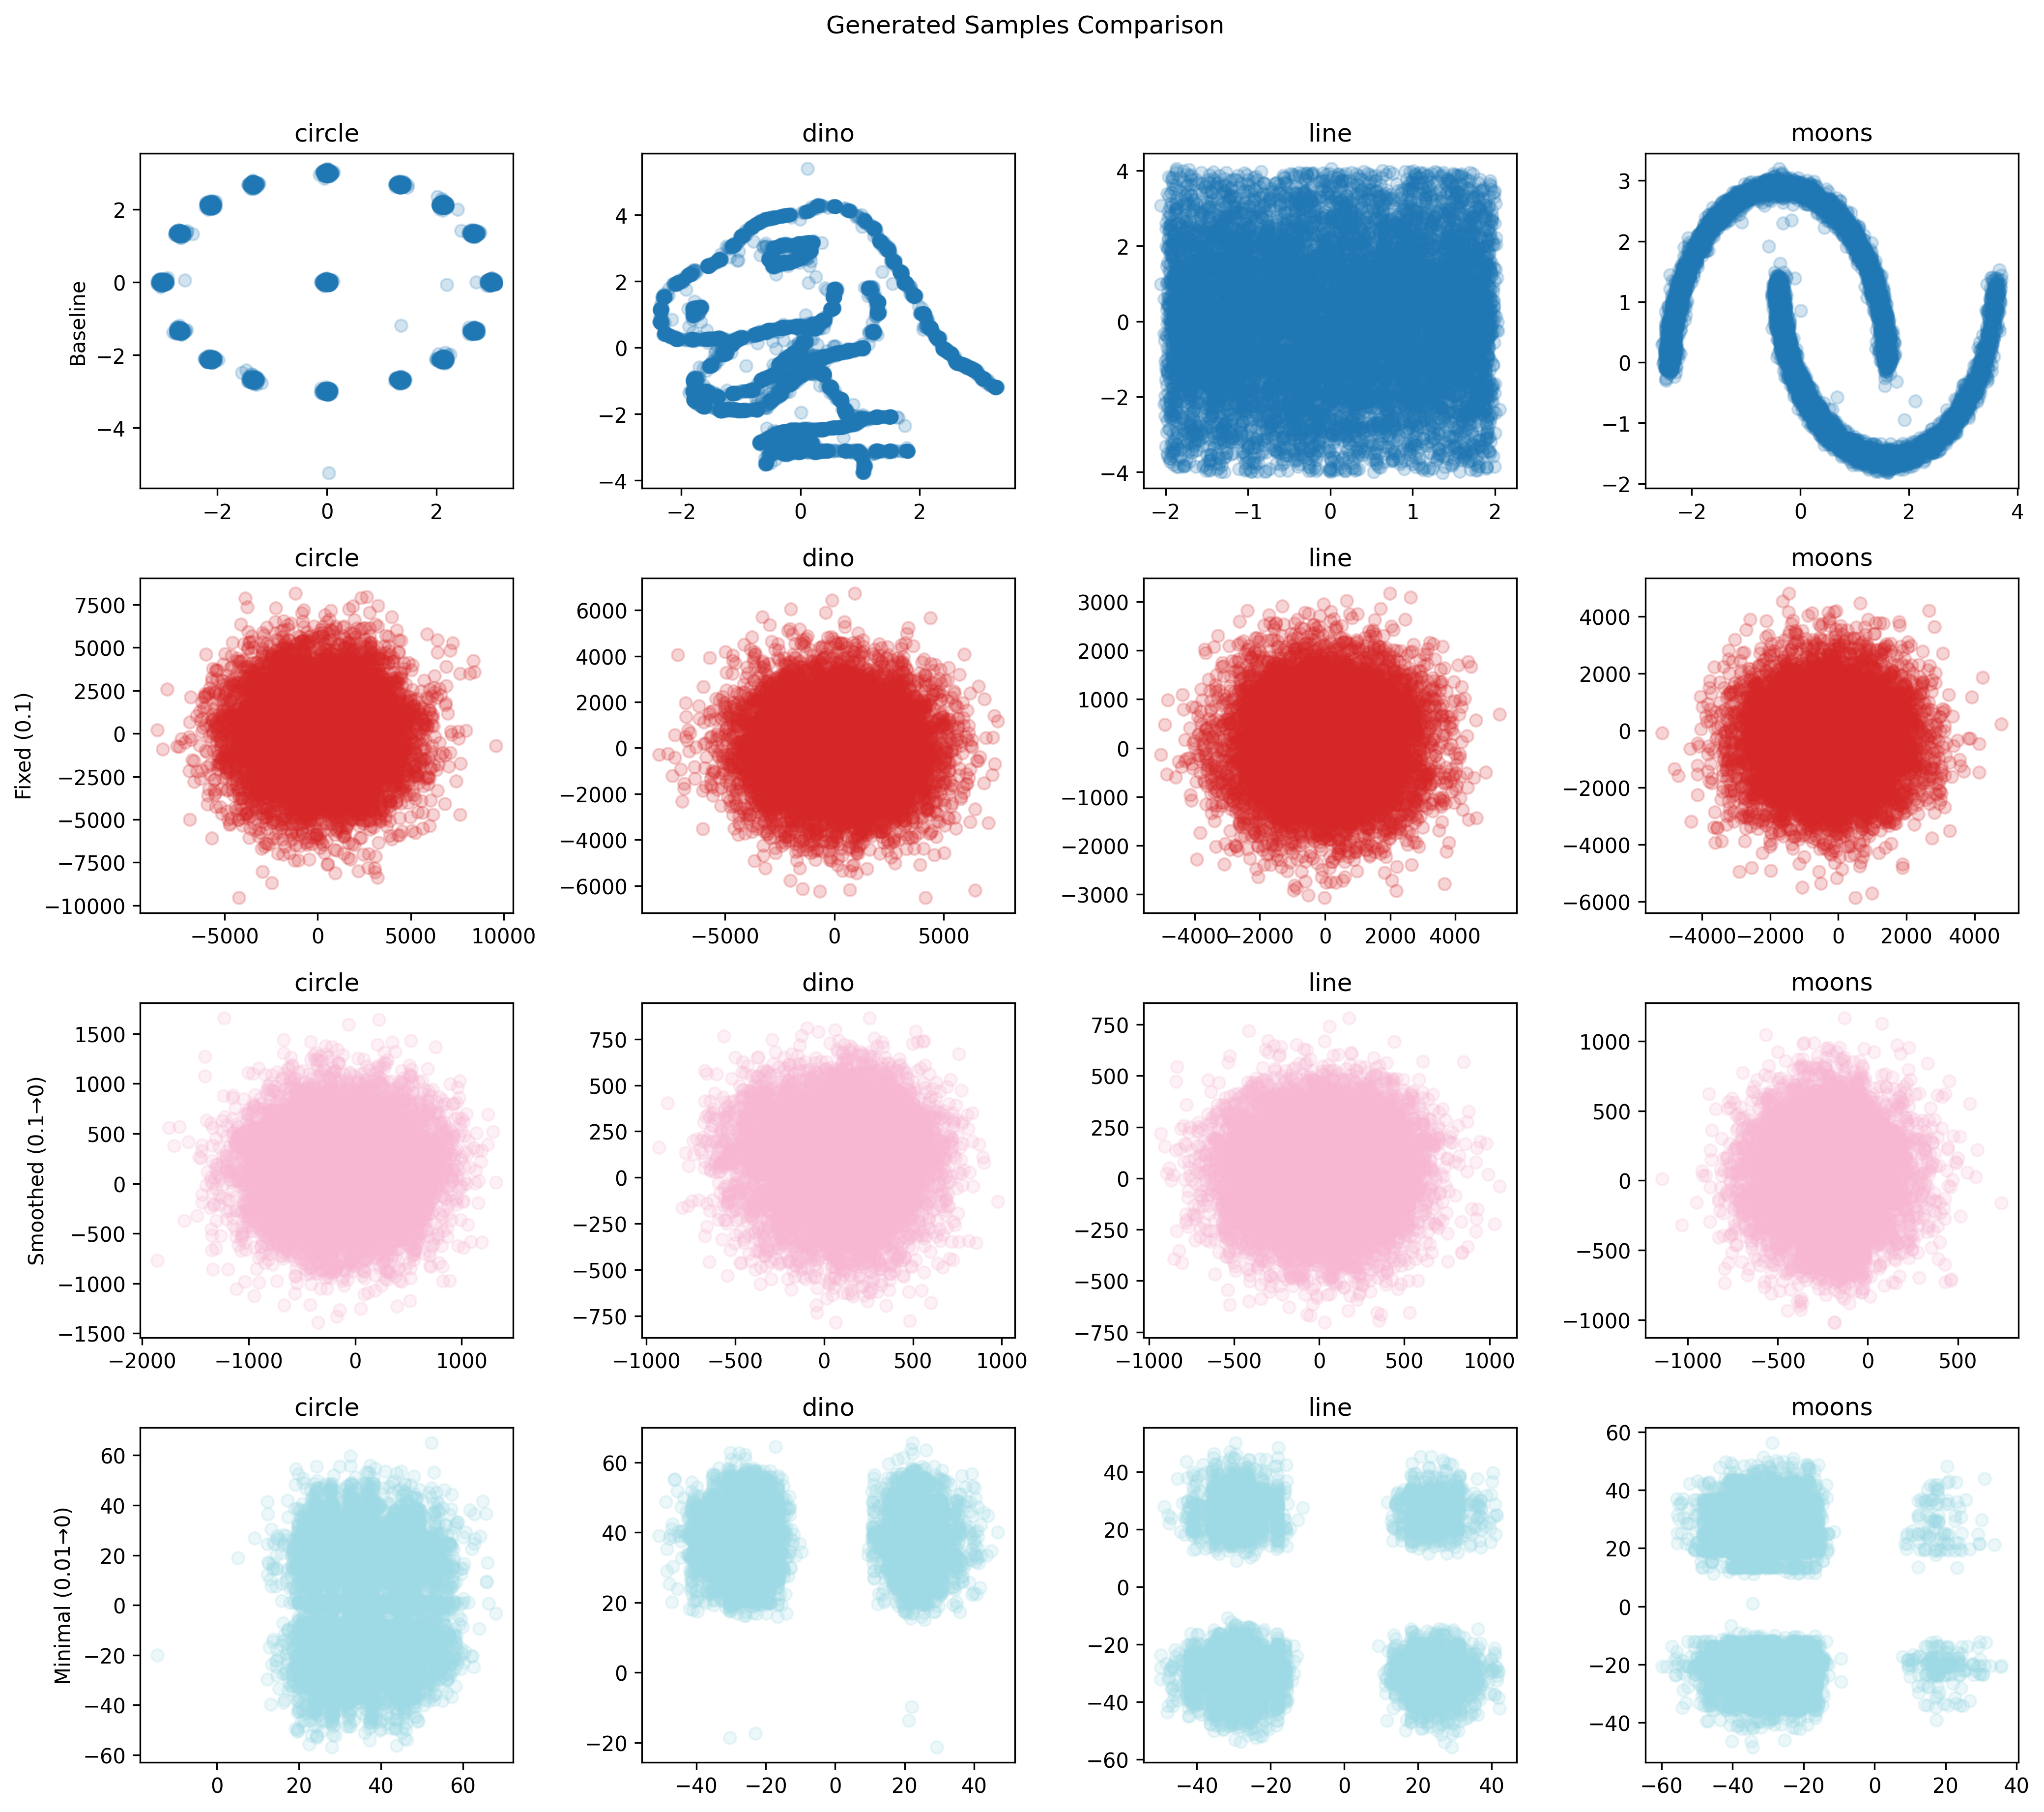
\includegraphics[width=0.98\textwidth]{generated_samples.png}
\caption{Generated samples comparison. Top: baseline. Bottom: guided variants showing artifacts and density distortions.}
\label{fig:generated_samples}
\end{figure}

\begin{figure}[t]
\centering
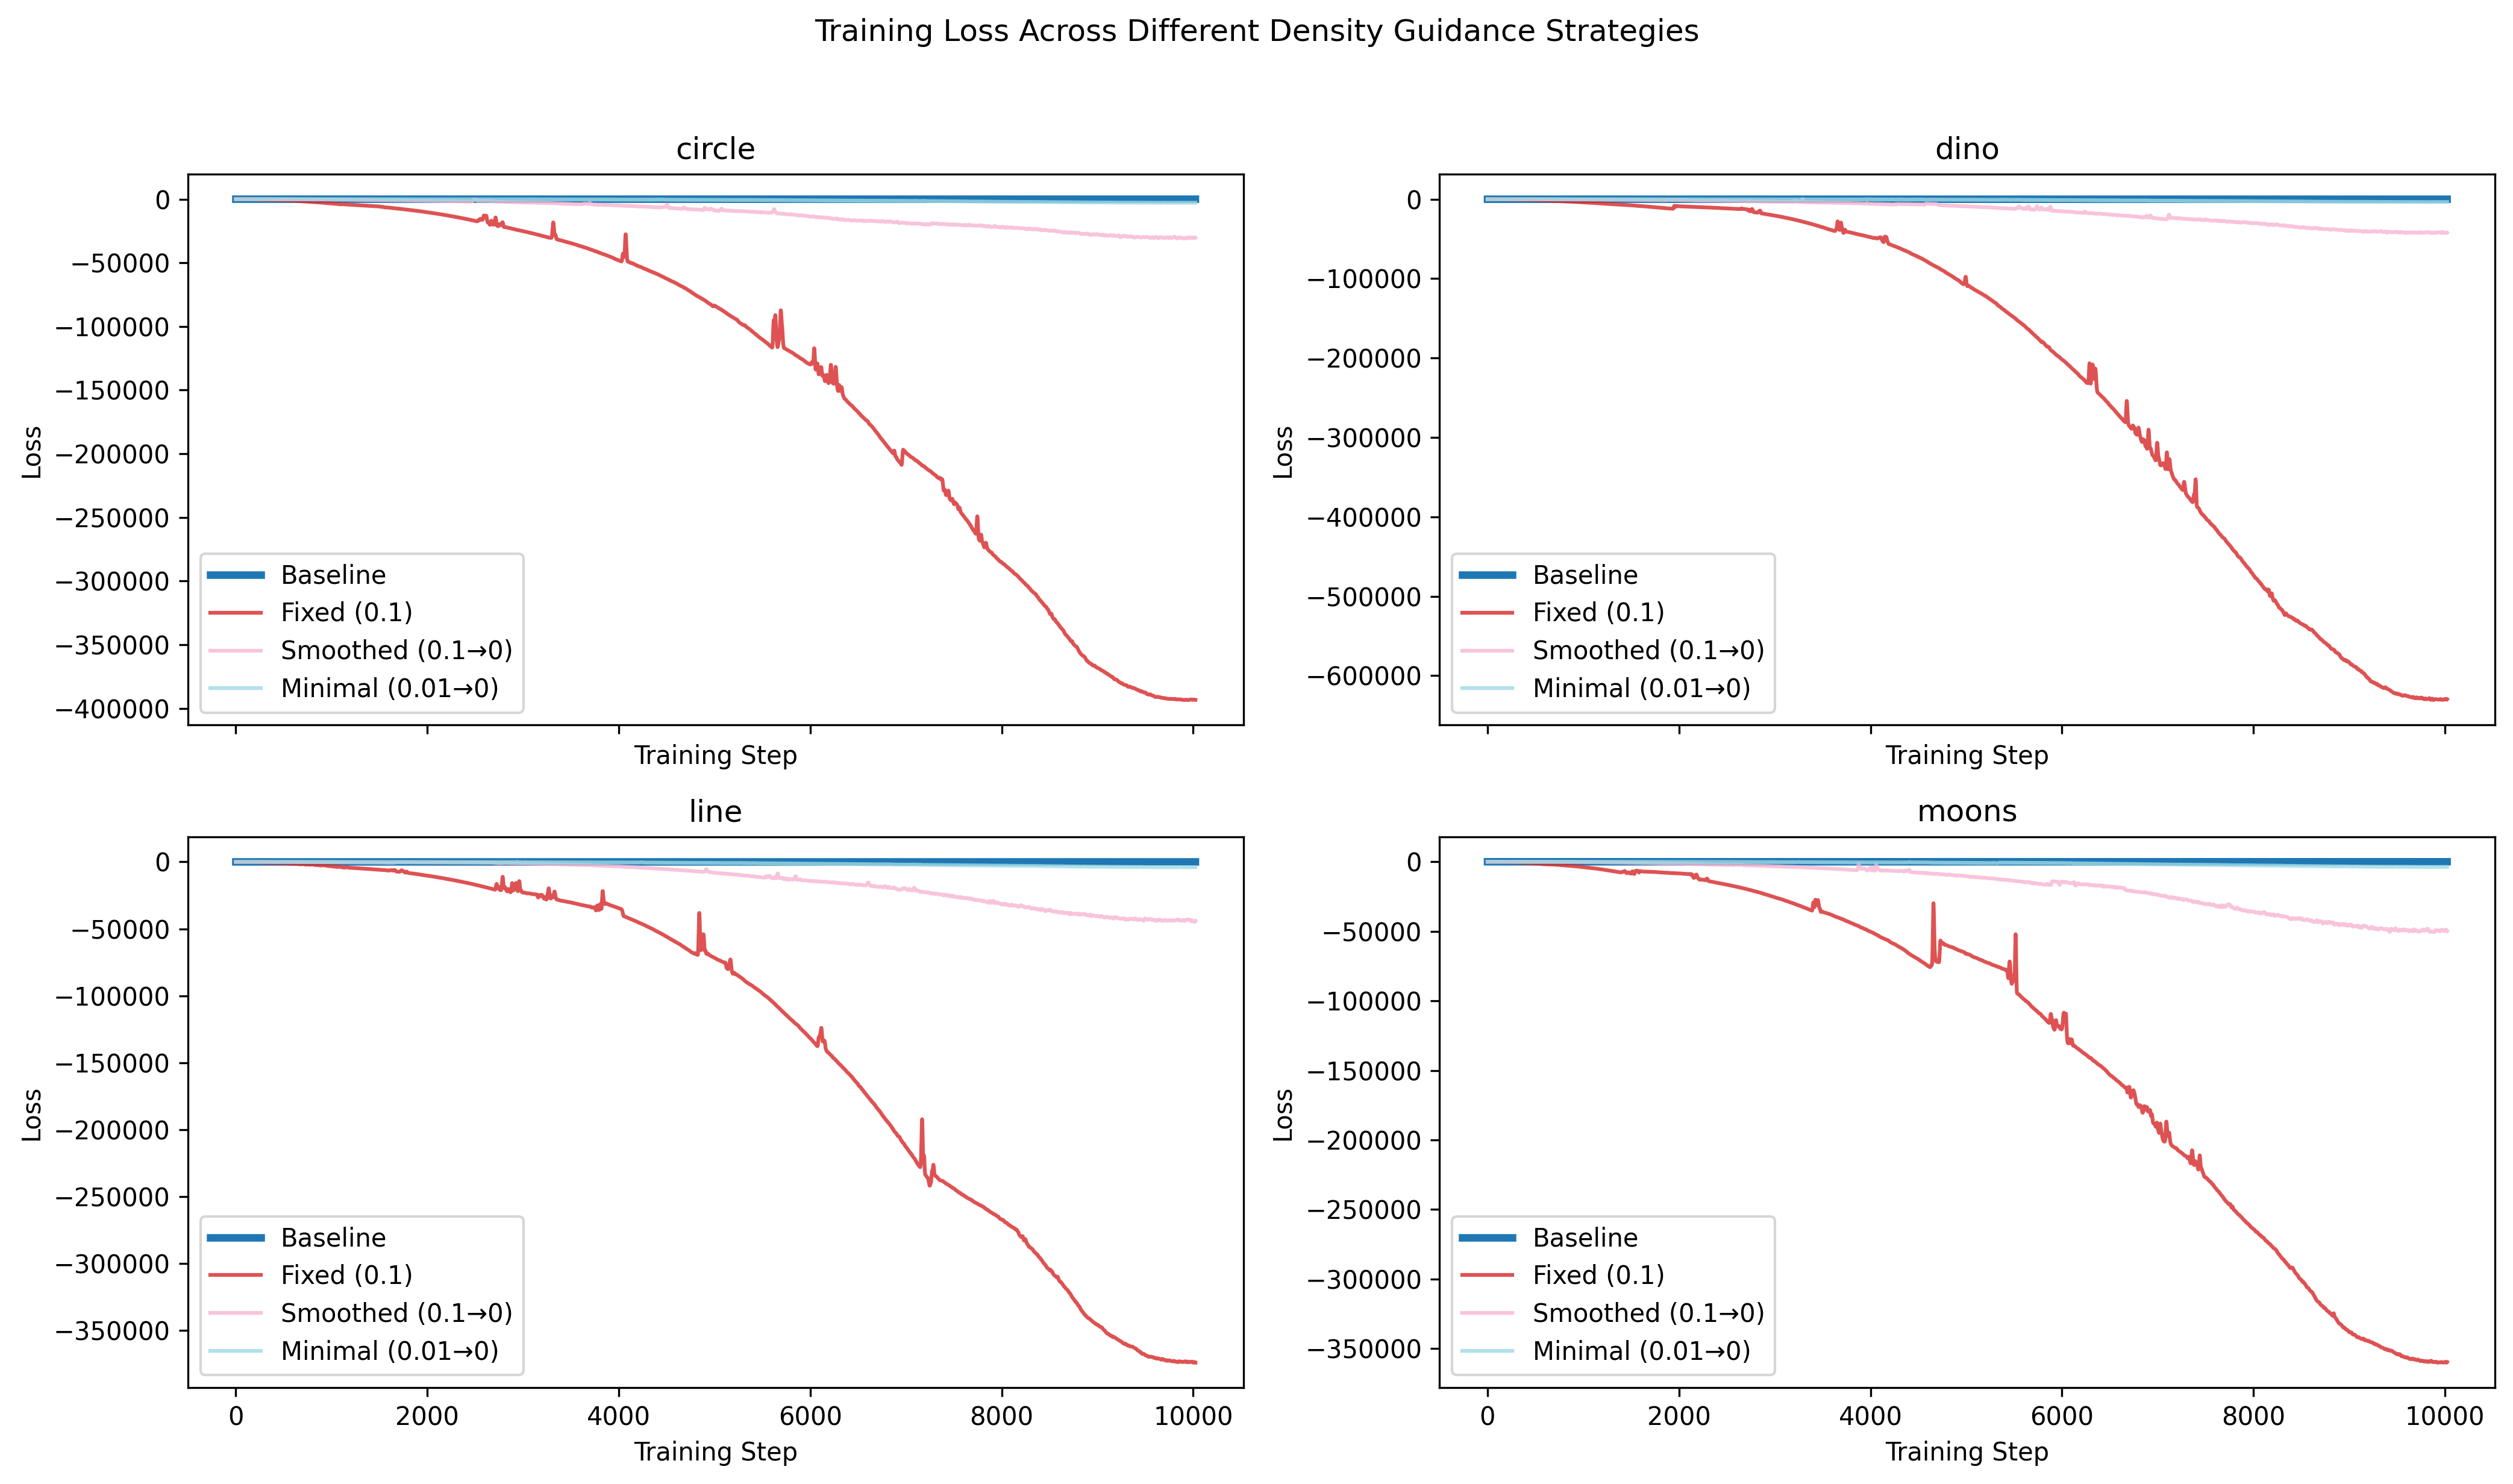
\includegraphics[width=0.98\textwidth]{train_loss.png}
\caption{Training loss curves. Baseline (black) shows faster convergence and lower final loss than guided variants.}
\label{fig:train_loss}
\end{figure}

\section{Conclusions and Future Work}
\label{sec:conclusion}

Our systematic evaluation yields three key insights about density-guided diffusion sampling:

\begin{itemize}
    \item \textbf{Consistent degradation}: All guidance variants increased KL divergence 15--25$\times$ while slowing inference 2--3$\times$, with no configuration outperforming baseline
    \item \textbf{Fundamental conflict}: The negative results across datasets and strategies suggest density estimation inherently disrupts diffusion dynamics
    \item \textbf{Practical implications}: Density guidance should be avoided despite its theoretical appeal
\end{itemize}

These findings challenge the assumption that density-aware sampling improves coverage, demonstrating instead that it systematically degrades performance. Our results align with recent theoretical work \citep{Aithal2024UnderstandingHI} showing diffusion models' sensitivity to sampling perturbations.

Future research directions include:
\begin{itemize}
    \item \textbf{Alternative objectives}: Distance metrics or diversity losses instead of density
    \item \textbf{Architectural solutions}: Modified denoisers that inherently promote coverage
    \item \textbf{Theoretical analysis}: Formal characterization of why density guidance fails
    \item \textbf{Hybrid approaches}: Combining diffusion with other generative paradigms \citep{vae,gan}
\end{itemize}

This work serves as a cautionary case study about the importance of empirical validation for theoretically-motivated modifications \citep{yang2023diffusion}. While elegant in principle, density guidance proves ineffective in practice, highlighting the need for alternative solutions to balanced sampling.

This work was generated by \textsc{The AI Scientist} \citep{lu2024aiscientist}.

\bibliographystyle{iclr2024_conference}
\bibliography{references}

\end{document}
